\chapter{Literature Review}

\section{Overview of Large Language Models}
    The evolution of LLMs can be traced back to earlier models of machine learning that attempted to process and understand language. However, it was the introduction of models like Google's BERT (Bidirectional Encoder Representations from Transformers) and OpenAI's GPT (Generative Pre-trained Transformer) series that marked a significant leap in the capabilities of language models. Each iteration of these models has brought about improvements in understanding context, generating text, and general language comprehension, culminating in state-of-the-art models that are capable of writing essays, composing poetry, and even generating code.
    

\section{Previous Studies on LLM Compression and Optimization}
    % Over the past few years, researchers have explored various techniques to optimize LLMs, focusing on model compression, parameter sharing, and other strategies to reduce computational overhead and improve efficiency. These studies have highlighted the importance of maintaining task-specific performance while enhancing the model's operational characteristics.
    % This section provides an overview of some key studies in the field of LLM optimization, focusing on the methodologies employed and the outcomes achieved.
    % \vspace*{0.2cm}

    Over the past few years, the increasing demand for Large Language Models (LLMs) across a vast spectrum of applications, from natural language processing to content generation, has underscored the critical need for optimization strategies tailored to these complex systems. Researchers have delved into a variety of optimization techniques aimed at refining LLMs, with a keen focus on enhancing model efficiency and reducing the computational burden without compromising the specialized performance that these models are known for. 
    Key areas of investigation have included model compression, prompt engineering, and other innovative approaches, all geared towards optimizing resource utilization and facilitating wider accessibility and deployment of LLMs in real-world scenarios. This section aims to shed light on seminal contributions to the optimization of LLMs, detailing the inventive methodologies adopted and the significant advancements realized in making these models more efficient and adaptable to the ever-evolving demands of technology and society.
    
    % \subsection*{Full Fine-Tuning}
    %     One of the traditional approaches to adapting large pre-trained models to specific tasks is full fine-tuning, where the entire model is retrained on the target dataset. While effective, this method is computationally expensive and time-consuming, requiring significant resources to achieve optimal performance. Moreover, fine-tuning can lead to catastrophic forgetting, where the model loses previously acquired knowledge during the adaptation process.
    
    \subsection{Low-Memory Optimization}
        % Although current methods have primarily concentrated on fine-tuning in a parameter-efficient manner, adjusting or augmenting only a minimal number of parameters, there has been little focus on the challenge of comprehensively fine-tuning all parameters of Large Language Models (LLMs) within the constraints of limited resources. 
        % This is what \cite{lv2023parameter} aims to address by proposing a novel optimization technique that combines gradient computation and parameter update in a single step to reduce memory usage during fine-tuning. The proposed method, named \textbf{LO}w-\textbf{M}emory \textbf{O}ptimization (LOMO), significantly reduces the memory footprint required for fine-tuning LLMs, making it feasible to full fine-tune large models on resource-constrained devices without compromising performance.
        % \\
        % In detail, they take Stochastic Gradient Descent (SDG) as the optimizer, and they express the vanilla gradient descent as \(\text{grad} = \frac{\partial \mathcal{L}}{\partial p}\) , \(p = p - lr * \text{grad}\), which is a
        % two-step process, computing the gradients first and updating it to the parameters. The fusion version is \(p = p - lr * \frac{\partial \mathcal{L}}{\partial p}\).
        % \\
        % The experiments conducted on ... demonstrates that LOMO \\

        In addressing the optimization of LLMs with constrained resources, \cite{lv2023parameter} presents a pioneering approach named \textbf{LO}w-\textbf{M}emory \textbf{O}ptimization (LOMO). This method innovates by fusing gradient computation and parameter update into a single operation, significantly reducing the memory requirements for full model fine-tuning. Notably, LOMO enables the comprehensive fine-tuning of models with up to 65 billion parameters on hardware as accessible as a single setup equipped with 8 RTX 3090 GPUs.

        A critical innovation within LOMO is the application of Stochastic Gradient Descent (SGD) as the optimizer, distinguished by its lack of reliance on intermediate state storage, thereby contributing to reduced memory consumption. Specifically, LOMO simplifies the traditional two-step process of gradient descent (\(\text{grad} = \frac{\partial \mathcal{L}}{\partial p}\), \(p = p - lr * \text{grad}\)) into a single-step process (\(p = p - lr * \frac{\partial \mathcal{L}}{\partial p}\)). This optimization not only minimizes memory usage but also maintains, or in some cases, enhances the fine-tuning efficacy for downstream tasks.

        The empirical evaluation of LOMO, particularly on the SuperGLUE benchmark, showcases its effectiveness in lowering memory requirements while preserving or improving model performance on various NLP tasks. The advancements brought forth by LOMO significantly democratize the process of fine-tuning LLMs, reducing the computational barrier and facilitating broader research and application possibilities in the field of Natural Language Processing.

    \subsection{Optimization by Prompting}
        Optimization by PROmpting (OPRO), as introduced by \cite{yang2023large}, represents a novel methodology for leveraging Large Language Models (LLMs) as optimizers. The core concept involves using the generative capabilities of LLMs to iteratively generate candidate solutions to optimization problems described in natural language. This process is guided by a meta-prompt, which provides the LLM with a concise description of the optimization task, historical performance data of past solutions, and a directive to generate new solutions aimed at optimizing the given objective function.
        
        The OPRO framework's approach to generating solutions is iterative and dynamic, enabling a detailed exploration and exploitation of the solution space. Each round of solution generation takes into account the performance trajectory of previous solutions, allowing the LLM to refine its approach continuously and hone in on more promising solution regions. This method allows for a sophisticated balance between exploring new solution avenues and exploiting known high-potential areas, a balance that is crucial for the success of any optimization process.
        
        Despite its innovative approach and promising results across various optimization tasks, the study acknowledges several limitations of the OPRO framework. The effectiveness of the optimization process is highly dependent on the quality and detail of the meta-prompt and the relevance and robustness of the initial solutions provided. Moreover, the computational demands of the iterative solution generation process, particularly for complex problems requiring numerous iterations for convergence, present significant challenges. These factors underscore the need for further research and development to refine the OPRO framework, focusing on improving prompt design, solution evaluation mechanisms, and computational efficiency to broaden its applicability and effectiveness in solving a wide range of optimization problems.
        
    % \subsection{Low-Rank Adaptation (LoRA)}
    %     Low-Rank Adaptation (LoRA) introduces an efficient technique for adapting large pre-trained models like GPT-3 to specific tasks without the need for extensive retraining of all model parameters. This approach leverages the observation that despite the high parameter count in large neural models, their effective operational space often exhibits a significantly lower intrinsic dimensionality.

    %     \paragraph{Theoretical Foundation}
    %     At the core of LoRA is the adaptation of weight matrices \(W \in \mathbb{R}^{d \times k}\) through the introduction of low-rank matrices \(A \in \mathbb{R}^{r \times k}\) and \(B \in \mathbb{R}^{d \times r}\), where \(r \ll \min(d,k)\). This results in the adapted weight matrix \(W'\) being represented as:
    %     \begin{equation}
    %         W' = W + BA = W + \Delta W
    %     \end{equation}
    %     Here, \(r\) denotes the rank and serves as a crucial parameter that balances the efficiency and expressiveness of the adaptation. This formulation ensures that the pre-trained weights (\(W\)) remain unchanged, preserving the foundational knowledge acquired during pre-training, while \(A\) and \(B\) encapsulate the task-specific adjustments.

    %     \paragraph{Advantages}
    %     LoRA's methodology brings forth several advantages:
    %     \begin{itemize}
    %         \item \textbf{Parameter Efficiency:} By optimizing the low-rank matrices \(A\) and \(B\), LoRA significantly reduces the number of trainable parameters, leading to efficient storage and faster adaptation processes. This is due to \(r\) being much smaller than both \(d\) and \(k\), so the total number of parameters in \(A\) and \(B\) combined \((r \times (d + k))\) is much less than the number of parameters in \(W\) \((d \times k)\).
    %         \item \textbf{Preservation of Pre-trained Knowledge:} The approach ensures that the valuable knowledge captured in the pre-trained model is retained, making it particularly beneficial for adapting computationally expensive models like GPT-3.
    %         \item \textbf{Flexibility and Scalability:} LoRA's adaptive process is highly scalable and flexible, making it possible to adapt large models to various tasks with minimal computational overhead.
    %     \end{itemize}

    %     \paragraph{Practical Implementation}
    %     Implementing LoRA involves selecting the transformer layers most relevant to the target task and applying the low-rank adaptations. The process requires initializing \(A\) and \(B\), choosing an appropriate rank \(r\), and training these matrices while keeping the rest of the model parameters fixed. This strategy allows for the efficient adaptation of large-scale models to specific tasks, significantly reducing the need for computational resources compared to traditional full model retraining.

\section{Evaluating Summarization with ROUGE}
    The evaluation of automated summarization models is crucial for assessing their efficiency and effectiveness in capturing the essence of text data. ROUGE, which stands for Recall-Oriented Understudy for Gisting Evaluation, provides a set of metrics that are indispensable for this purpose. Introduced by \cite{lin-2004-rouge}, ROUGE measures compare the overlap between computer-generated summaries and a set of reference summaries typically created by humans.

    \paragraph{ROUGE Metrics}
    ROUGE includes several specific metrics, such as ROUGE-N (n-gram overlap) and ROUGE-L (longest common subsequence), each suited for different aspects of summarization. For instance, ROUGE-N focuses on the exactness of content at various n-gram levels, providing insights into the precision of the summarization model in replicating key information. In contrast, ROUGE-L assesses the fluency and structure of the generated summaries by measuring sequence similarity, which is crucial for evaluating the narrative flow of the text.

    \paragraph{Application and Relevance}
    The application of ROUGE in evaluation has been extensively validated across various tasks, including the Document Understanding Conferences (DUC), where it has been used to measure the performance of summarization systems in a competitive environment. These metrics have proven to be reliable indicators of human judgment, making them a standard against which the summarization capabilities of LLMs are benchmarked. The relevance of ROUGE scores lies in their ability to provide quantifiable measures that correlate strongly with human evaluations, thus facilitating the improvement and development of more efficient summarization models.

    \paragraph{Significance in LLM Research}
    In the context of Large Language Models, understanding the effectiveness of different compression and optimization techniques often relies on the ability to evaluate how well the reduced models can summarize content. ROUGE metrics serve this purpose by quantifying the trade-offs between model complexity and performance retention, helping researchers and developers optimize LLMs without significant loss in functionality.

\chapter{Literature Review}

\section{Overview of Large Language Models}
The evolution of LLMs can be traced back to earlier models of machine learning that attempted to process and understand language. However, it was the introduction of models like Google's BERT (Bidirectional Encoder Representations from Transformers) and OpenAI's GPT (Generative Pre-trained Transformer) series that marked a significant leap in the capabilities of language models. Each iteration of these models has brought about improvements in understanding context, generating text, and general language comprehension, culminating in state-of-the-art models that are capable of writing essays, composing poetry, and even generating code.

\section{Previous Studies on LLM Compression}
    Over the past few year, the increasing demand for Large Language Models (LLMs) across a vast spectrum of applications, from natural language processing to content generation, has underscored the critical need for optimization strategies tailored to these complex systems. Researchers have delved into a variety of optimization techniques aimed at refining LLMs, with a keen focus on enhancing model efficiency and reducing the computational burden without compromising the specialized performance that these models are known for.
    A key area of investigation has been model compression, which involves reducing the size and complexity of LLMs while maintaining their functionality and performance. \\
    %\cite{zhu2023survey} presents a recent comprehensive overview of model compression techniques specifically designed for LLMs. 

    \subsection*{Low Rank Approximation}
        In the realm of large language models (LLMs), low-rank approximation has gained substantial traction as a method to fine-tune and streamline models. It has been utilized in various implementations, notably in LORA (\cite{hu2021lora}) and its subsequent adaptations (\cite{valipour-etal-2023-dylora, zhang2023adaptive, chavan2024oneforall}). These adaptations focus on leveraging low-rank structures to optimize the performance of LLMs without extensive resource demands.
        
        A novel application of this technique is seen in TensorGPT (\cite{xu2023tensorgpt}), which employs a low-rank tensor format to manage large embeddings efficiently. By adopting the Tensor-Train Decomposition (TTD), TensorGPT not only reduces the spatial complexity of LLMs but also potentially boosts their deployment on edge devices. This method treats each token embedding as a Matrix Product State (MPS), enabling the compression of the embedding layer by up to a factor of \(38.40\). Remarkably, this compression is achieved without sacrificing, and in some cases even enhancing, the performance of the model compared to its original configuration.
        
        This focus on low-rank approximation underscores its critical role in advancing the field of LLMs by facilitating more efficient model architectures that maintain high performance while being computationally less demanding.
        

\section{Introduction to BART}
    \textbf{BART: Denoising Sequence-to-Sequence Pre-training for Natural Language Generation, Translation, and Comprehension} by (\cite{lewis2019bart}), introduces BART as a versatile pretraining approach for natural language processing tasks. BART combines the benefits of both autoregressive (like GPT) and autoencoding (like BERT) paradigms into a unified model.

    \subsection{Architecture and Training}
    BART employs a Transformer-based sequence-to-sequence architecture from 
    
    (\cite{vaswani2023attention}), utilizing a bidirectional encoder (similar to BERT) and a left-to-right decoder (similar to GPT) to handle a wide array of tasks from generation to comprehension. For the base model (BART-base) and the large model (BART-large), the encoder and decoder consist of \(6\) and \(12\) layers, respectively (Appendix \ref{appendix:BART}).
    It is trained through a novel denoising objective, where the model reconstructs the original text from corrupted versions. This involves techniques such as token masking (\cite{devlin2019bert}) and text infilling, enhancing the model's ability to understand and generate contextually rich language.
    \begin{figure}[H]
        \centering
        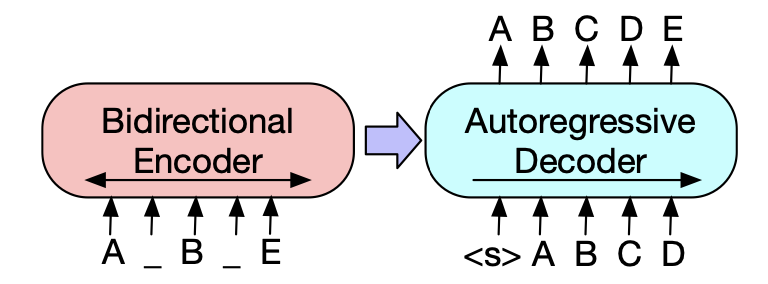
\includegraphics[width=0.8\textwidth]{figs/BART_architecture.png}
        \caption{BART model's processing mechanism - Taken from \cite{lewis2019bart}}
        \label{fig:bart_process}
    \end{figure}
    Figure \ref{fig:bart_process} illustrates the BART model's processing mechanism. The original text sequence [ABCDE] is transformed into a masked version [A[MASK]B[MASK]E]. BART's encoder learns bidirectional representations from this altered input, allowing it to handle inputs that are not aligned with decoder outputs. The decoder then attempts to reconstruct the original sequence autoregressively by optimizing the negative log-likelihood. For fine-tuning, the model processes an uncorrupted document to enhance accuracy and adaptability.
    \subsection{Efficacy and Applications}
    The versatility of BART is demonstrated across various NLP tasks including text generation, comprehension, and translation. Notably, BART outperforms previous work on benchmarks like ROUGE, showcasing substantial improvements particularly in abstractive summarization tasks. The model's ability to fine-tune to specific tasks using pre-trained weights allows it to excel in both generation and comprehension roles, making it a powerful tool for a broad range of applications.

\section{Evaluating Summarization with ROUGE}\label{sec:rouge}
The evaluation of automated summarization models is crucial for assessing their efficiency and effectiveness in capturing the essence of text data. ROUGE (\cite{lin-2004-rouge}), which stands for Recall-Oriented Understudy for Gisting Evaluation, provides a set of metrics that are indispensable for this purpose. Introduced by \cite{lin-2004-rouge}, ROUGE measures compare the overlap between computer-generated summaries and a set of reference summaries typically created by humans.

\paragraph{ROUGE Metrics}
ROUGE includes several specific metrics, such as ROUGE-N (n-gram overlap) and ROUGE-L (longest common subsequence), each suited for different aspects of summarization. For instance, ROUGE-N focuses on the exactness of content at various n-gram levels, providing insights into the precision of the summarization model in replicating key information. In contrast, ROUGE-L assesses the fluency and structure of the generated summaries by measuring sequence similarity, which is crucial for evaluating the narrative flow of the text.

\paragraph{Application and Relevance}
The application of ROUGE in evaluation has been extensively validated across various tasks, including the Document Understanding Conferences (DUC), where it has been used to measure the performance of summarization systems in a competitive environment. These metrics have proven to be reliable indicators of human judgment, making them a standard against which the summarization capabilities of LLMs are benchmarked. The relevance of ROUGE scores lies in their ability to provide quantifiable measures that correlate strongly with human evaluations, thus facilitating the improvement and development of more efficient summarization models.

\paragraph{Significance in LLM Research}
In the context of Large Language Models, understanding the effectiveness of different compression and optimization techniques often relies on the ability to evaluate how well the reduced models can summarize content. ROUGE metrics serve this purpose by quantifying the trade-offs between model complexity and performance retention, helping researchers and developers optimize LLMs without significant loss in functionality.
